\iffalse
\documentclass[journal,10pt,twocolumn]{article}
\usepackage{graphicx}
\usepackage[margin=0.5in]{geometry}
\usepackage[cmex10]{amsmath}
\usepackage{array}
\usepackage{booktabs}
\usepackage{mathtools}
\title{\textbf{Conic section Assignment}}
\author{Maddu Dinesh}
\date{September 2022}


\providecommand{\norm}[1]{\left\lVert#1\right\rVert}
\providecommand{\abs}[1]{\left\vert#1\right\vert}
\let\vec\mathbf
\newcommand{\myvec}[1]{\ensuremath{\begin{pmatrix}#1\end{pmatrix}}}
\newcommand{\mydet}[1]{\ensuremath{\begin{vmatrix}#1\end{vmatrix}}}
\providecommand{\brak}[1]{\ensuremath{\left(#1\right)}}
\providecommand{\lbrak}[1]{\ensuremath{\left(#1\right.}}
\providecommand{\rbrak}[1]{\ensuremath{\left.#1\right)}}
\providecommand{\sbrak}[1]{\ensuremath{{}\left[#1\right]}}

\begin{document}

\maketitle
\paragraph{\textit{Problem Statement} -
\fi
Find the area of the region bounded by the curve $y^2=x$ and the lines $x=1$ and $x=4$ and the axis in the first quadrant.
	\begin{figure}[!h]
		\centering
 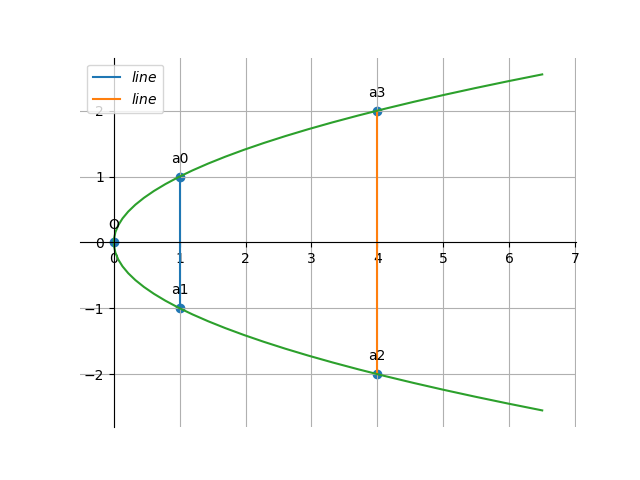
\includegraphics[width=\columnwidth]{chapters/12/8/1/1/figs/conics1.png}
		\caption{}
		\label{fig:12/8/1/1}
  	\end{figure}
	\\
	\solution

\iffalse
\section*{\large Solution}

\begin{figure}[h]
\centering
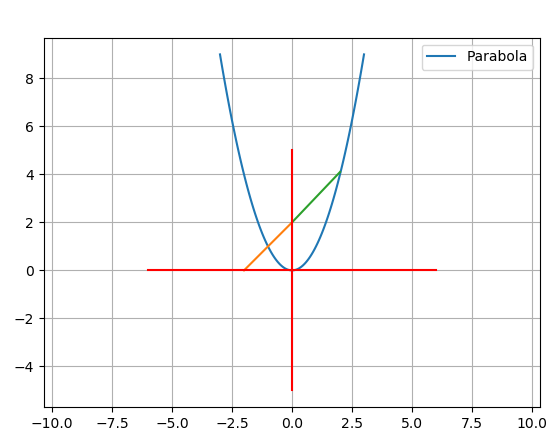
\includegraphics[width=1\columnwidth]{conics1.png}

\caption{The parabola formed by the curve $y^2 = x$ and the lines x=1 and x=4}
\label{fig:parabola}
\end{figure}

The given equation of parabola $y^2 = x$ can be written in the general quadratic form as
\begin{align}
    \label{eq:conic_quad_form}
    \vec{x}^{\top}\vec{V}\vec{x}+2\vec{u}^{\top}\vec{x}+f=0
    \end{align}
where
%
\fi
The parameters of the conic are
\begin{align}
	\vec{V} = \myvec{0 & 0\\0 & 1},
	\vec{u} = -\frac{1}{2}\myvec{ 1\\0},
	f = 0
	%\\
\end{align}
\iffalse
The point of intersection of the lines $x=1$ and $x=4$ to the parabola is given by


The points of intersection of the line 
\begin{align}
	L: \quad \vec{x} = \vec{q} + \mu \vec{m} \quad \mu \in \mathbf{R}
\label{eq:conic_tangent}
\end{align}
with the conic section are given by
\begin{align}
\vec{x}_i = \vec{q} + \mu_i \vec{m}
\label{eq:conic_tangent_pts}
\end{align}
%
where
{\tiny
\begin{multline}
\mu_i = \frac{1}
{
\vec{m}^T\vec{V}\vec{m}
}
\lbrak{-\vec{m}^T\brak{\vec{V}\vec{q}+\vec{u}}}
\\
\pm
\rbrak{\sqrt{
\sbrak{
\vec{m}^T\brak{\vec{V}\vec{q}+\vec{u}}
}^2
-
\brak
{
\vec{q}^T\vec{V}\vec{q} + 2\vec{u}^T\vec{q} +f
}
\brak{\vec{m}^T\vec{V}\vec{m}}
}
}
\label{eq:tangent_roots}
\end{multline}
}
\fi
For the line $x-1=0$, the parameters are  
\begin{align}
	\vec{q}_2=\myvec{1\\0},
	\vec{m}_2=\myvec{0\\1}
\end{align}
Substituting from the above in 
\eqref{eq:tangent_roots},
\begin{align}
\mu_i=1,-1
\end{align}
yilelding 
the points of intersection 
\begin{align}
	\vec{a}_0=\myvec{1\\1},
	\vec{a}_1=\myvec{1\\-1}
\end{align}
Similarly, 
for the line $x-4=0$ 
\begin{align}
\vec{q_1}=\myvec{4\\0},
\vec{m_1}=\myvec{0\\1}
\end{align}
yielding
\begin{align}
\mu_i=2,-2
\end{align}
from which, the points of 
intersection are
\begin{align}
\vec{a_3}=\myvec{4\\2},
\vec{a_2}=\myvec{4\\-2}
\end{align}
Thus, 
the area of the parabola in between the lines $x=1$ and $x=4$ is given by
\begin{align}
\int_{0}^{4} \ \sqrt{x} \,dx-\int_{0}^{1} \ \sqrt{x} \,dx
=14/3
\end{align}
\iffalse


\section*{\large Construction}

{
\setlength\extrarowheight{5pt}
\begin{tabular}{|l|c|}
    \hline 
    \textbf{Points} & \textbf{intersection points} \\ \hline
	a0 & $\myvec{
   1\\
   1
   } $ \\\hline
	a1 & $\myvec{
   1\\
   -1
   } $ \\\hline
    
	a3 & $\myvec{
   4\\
   2
   } $ \\\hline
	a2 & $\myvec{
   4\\
   -2
   } $ \\\hline
      
      \end{tabular}
}

\end{document}
\fi
